\documentclass[11pt,twoside,titlepage]{article}
\usepackage[tc]{titlepic}
\usepackage{times}
\usepackage{float}
\usepackage{amssymb}
\usepackage{amsmath}
\usepackage{amsthm}
\usepackage{needspace}
\usepackage{url}
\usepackage{hyperref}
%\usepackage{mathptm}
\usepackage{fancyhdr}
\usepackage{wrapfig}
\ifx\pdfoutput\undefined
% we are running LaTeX, not pdflatex
\usepackage{epsfig,color}
\else
% we are running pdflatex, so convert .eps files to .pdf
\usepackage[pdftex]{epsfig,color}
\usepackage{epstopdf}
\usepackage{pdfsync}
\fi
\usepackage{ifthen,version}
\usepackage{listings}
%\usepackage{temporal}
%\usepackage{algorithmic}
%\newboolean{print-solutions}

% Start of configuration section
% Comment out the following line to exclude the printing of solutions.
%\setboolean{print-solutions}{true}
%\newcommand{\labnumber}{1}
%\newcommand{\labname}{Digital Logic Gates}
\newcommand{\coursenumber}{Boot Camp How-To Document}
%\newcommand{\coursename}{Introduction to Digital Design}
% End of configuration section

% Conditional definitions
% \newcommand{\dateorsol}{\LARGE \ifthenelse{\boolean{print-solutions}}%
%   {Solutions}{Due \duedate}}
% %\newcommand{\headertxt}{\sl \ifthenelse{\boolean{print-solutions}}%
% %  {Solutions to}{} Laboratory Exercise \#\labnumber}
% \newcommand{\points}[1]{\ifthenelse{\boolean{print-solutions}}%
%   {}{[#1 points.]}}
% \ifthenelse{\boolean{print-solutions}}{\includeversion{prnt-solns}}%
% {\excludeversion{prnt-solns}}

\textwidth=7.25in
\evensidemargin=-0.35in
\oddsidemargin=-0.35in

\newcommand{\ite}{\operatorname{ite}}
\newcommand{\itec}{\operatorname{ite\_constant}}

{\theoremstyle{definition} \newtheorem{definition}{Definition}}
\newtheorem{theorem}{Theorem}
\newtheorem{lemma}{Lemma}
\newtheorem{corollary}{Corollary}
\newtheorem{proposition}{Proposition}
{\theoremstyle{remark}
  \newtheorem{example}{Example}
  \newtheorem{problem}{Problem}
  \newtheorem{note}{Note}}
% Fortunately, proofs can be nested.
\newenvironment{solution}{\begin{proof}[Solution]}{\end{proof}}


\newcommand{\ta}{Created By: Kunal Bharathi and Prof. Sunil P. Khatri\\August 2020}
\title{ \huge Department of Electrical and Computer Engineering\\ \huge Texas A\&M University \\}
\author{ \huge Windows for Mac Users (Boot Camp)\\ \\ \huge How-To Document \\ \\ \\ \ta}

\titlepic{
\includegraphics[width=0.5\textwidth]{logo}}

\date{}
\pagestyle{fancy}
\lhead[\rm\thepage]{\headertxt}
\rhead[\headertxt]{\rm\thepage}
\lfoot[]{\coursenumber}
%\cfoot{\instructor}
\rfoot[\coursenumber]{}

\begin{document}
\bibliographystyle{alpha}
\maketitle

\section{Introduction}

This guide is intended for students who use a Mac. Students registered for ECEN 248/449/749 will be using a tool called Vivado from Xilinx. Vivado is only available for Windows and Linux. If you are a Mac user, this document will help you set up an instance of the Windows 10 OS on your Mac, so you can install Vivado on this instance of Windows 10.\\
\\
\noindent
Using Apple's Boot Camp Assistant to install Windows 10 on your Mac will allow you to use both MacOS and Windows 10 on the same machine. This document is divided into three sections: 
\begin{itemize}
    \item Preparing to Install Windows 10
    \item Installing Windows 10 using Boot Camp Assistant
    \item Working with Windows and Mac on the same machine
\end{itemize}

\\

\noindent
\textbf{Note:} Before you begin the Boot Camp procedure, please read through the entire document carefully. This will help ensure that you have everything you need for a successful install.\\

\noindent
\textbf{Note:} There are some very helpful Boot Camp YouTube tutorials. Here is a link to one that guides you through the entire process from start to finish: https://www.youtube.com/watch?v=Hmm9Q-T0oTo
\\
\\
There will be minor variations from the YouTube video to what you see on your screen, therefore please do read this document.\\
\\
This guide was developed on a Mac running MacOS Catalina 10.15.5. You might see small variations in the options based on which version of MacOS you are running.

\section{Preparing to Install Windows 10}

In this section we will describe what you need to do before you start your Windows 10 installation. Here are the steps that we will be covering in this section:
\begin{itemize}

    \item Checking your Mac for compatibility
    \item Backing Up your Mac
    \item Obtaining a Windows 10 license and ISO
\end{itemize}

\subsection{Checking your Mac for compatibility}

Officially Apple's Boot Camp supports the following devices (if your device is not supported by Apple, STOP):

\begin{itemize}
    \item MacBook introduced in 2015 or later
    \item MacBook Air introduced in 2012 or later
    \item MacBook Pro introduced in 2012 or later
    \item Mac mini introduced in 2012 or later
    \item iMac introduced in 2012 or later
    \item iMac Pro (all models)
    \item Mac Pro introduced in 2013 or later
\end{itemize}

You also have to ensure that you have enough space on your disk to install Windows 10. According to Apple:

\begin{itemize}
    \item 64GB or more free storage space on your Mac startup disk (your SSD/HDD)
    \item Your Mac can have as little as 64GB of free storage space, but at least 128GB of free storage space provides the best experience. Automatic Windows updates require that much space or more
    \item If you have an iMac Pro or Mac Pro with 128GB of memory (RAM) or more, your startup disk needs at least as much free storage space as your Mac has memory
\end{itemize}

\noindent
Our recommendation is that you have at least 128 GB of space free for Windows 10. This will ensure enough space for later installing Vivado and also for Windows Updates.

\subsection{Backing Up Your Mac}

If you have determined that you have a Boot Camp compatible system, the next step is to back up your data. If something goes wrong during the installation, you do not want to loose any important information stored on your machine. There are different options for backing up data, some of them are:
\begin{itemize}
    \item Use Time-Machine (https://support.apple.com/en-us/HT201250)
    \item Copy all your important files to an external backup disk
    \item Upload a copy of your important files and folders to a service like DropBox or Google Drive
\end{itemize}

\noindent
Completing this backup step will protect you against any accidental loss of data.

\subsection{Obtaining a Windows 10 license and ISO}

\begin{figure}[htb]
	\centering 
	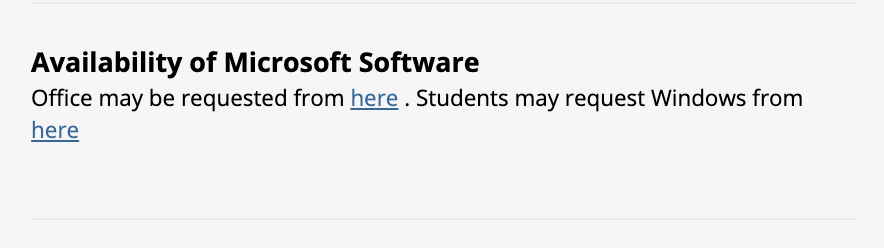
\includegraphics[ width=.8\textwidth]{oth}
	\caption{Link For Getting Microsoft Software}
	\label{oth}
\end{figure}

\begin{figure}[htb]
	\centering 
	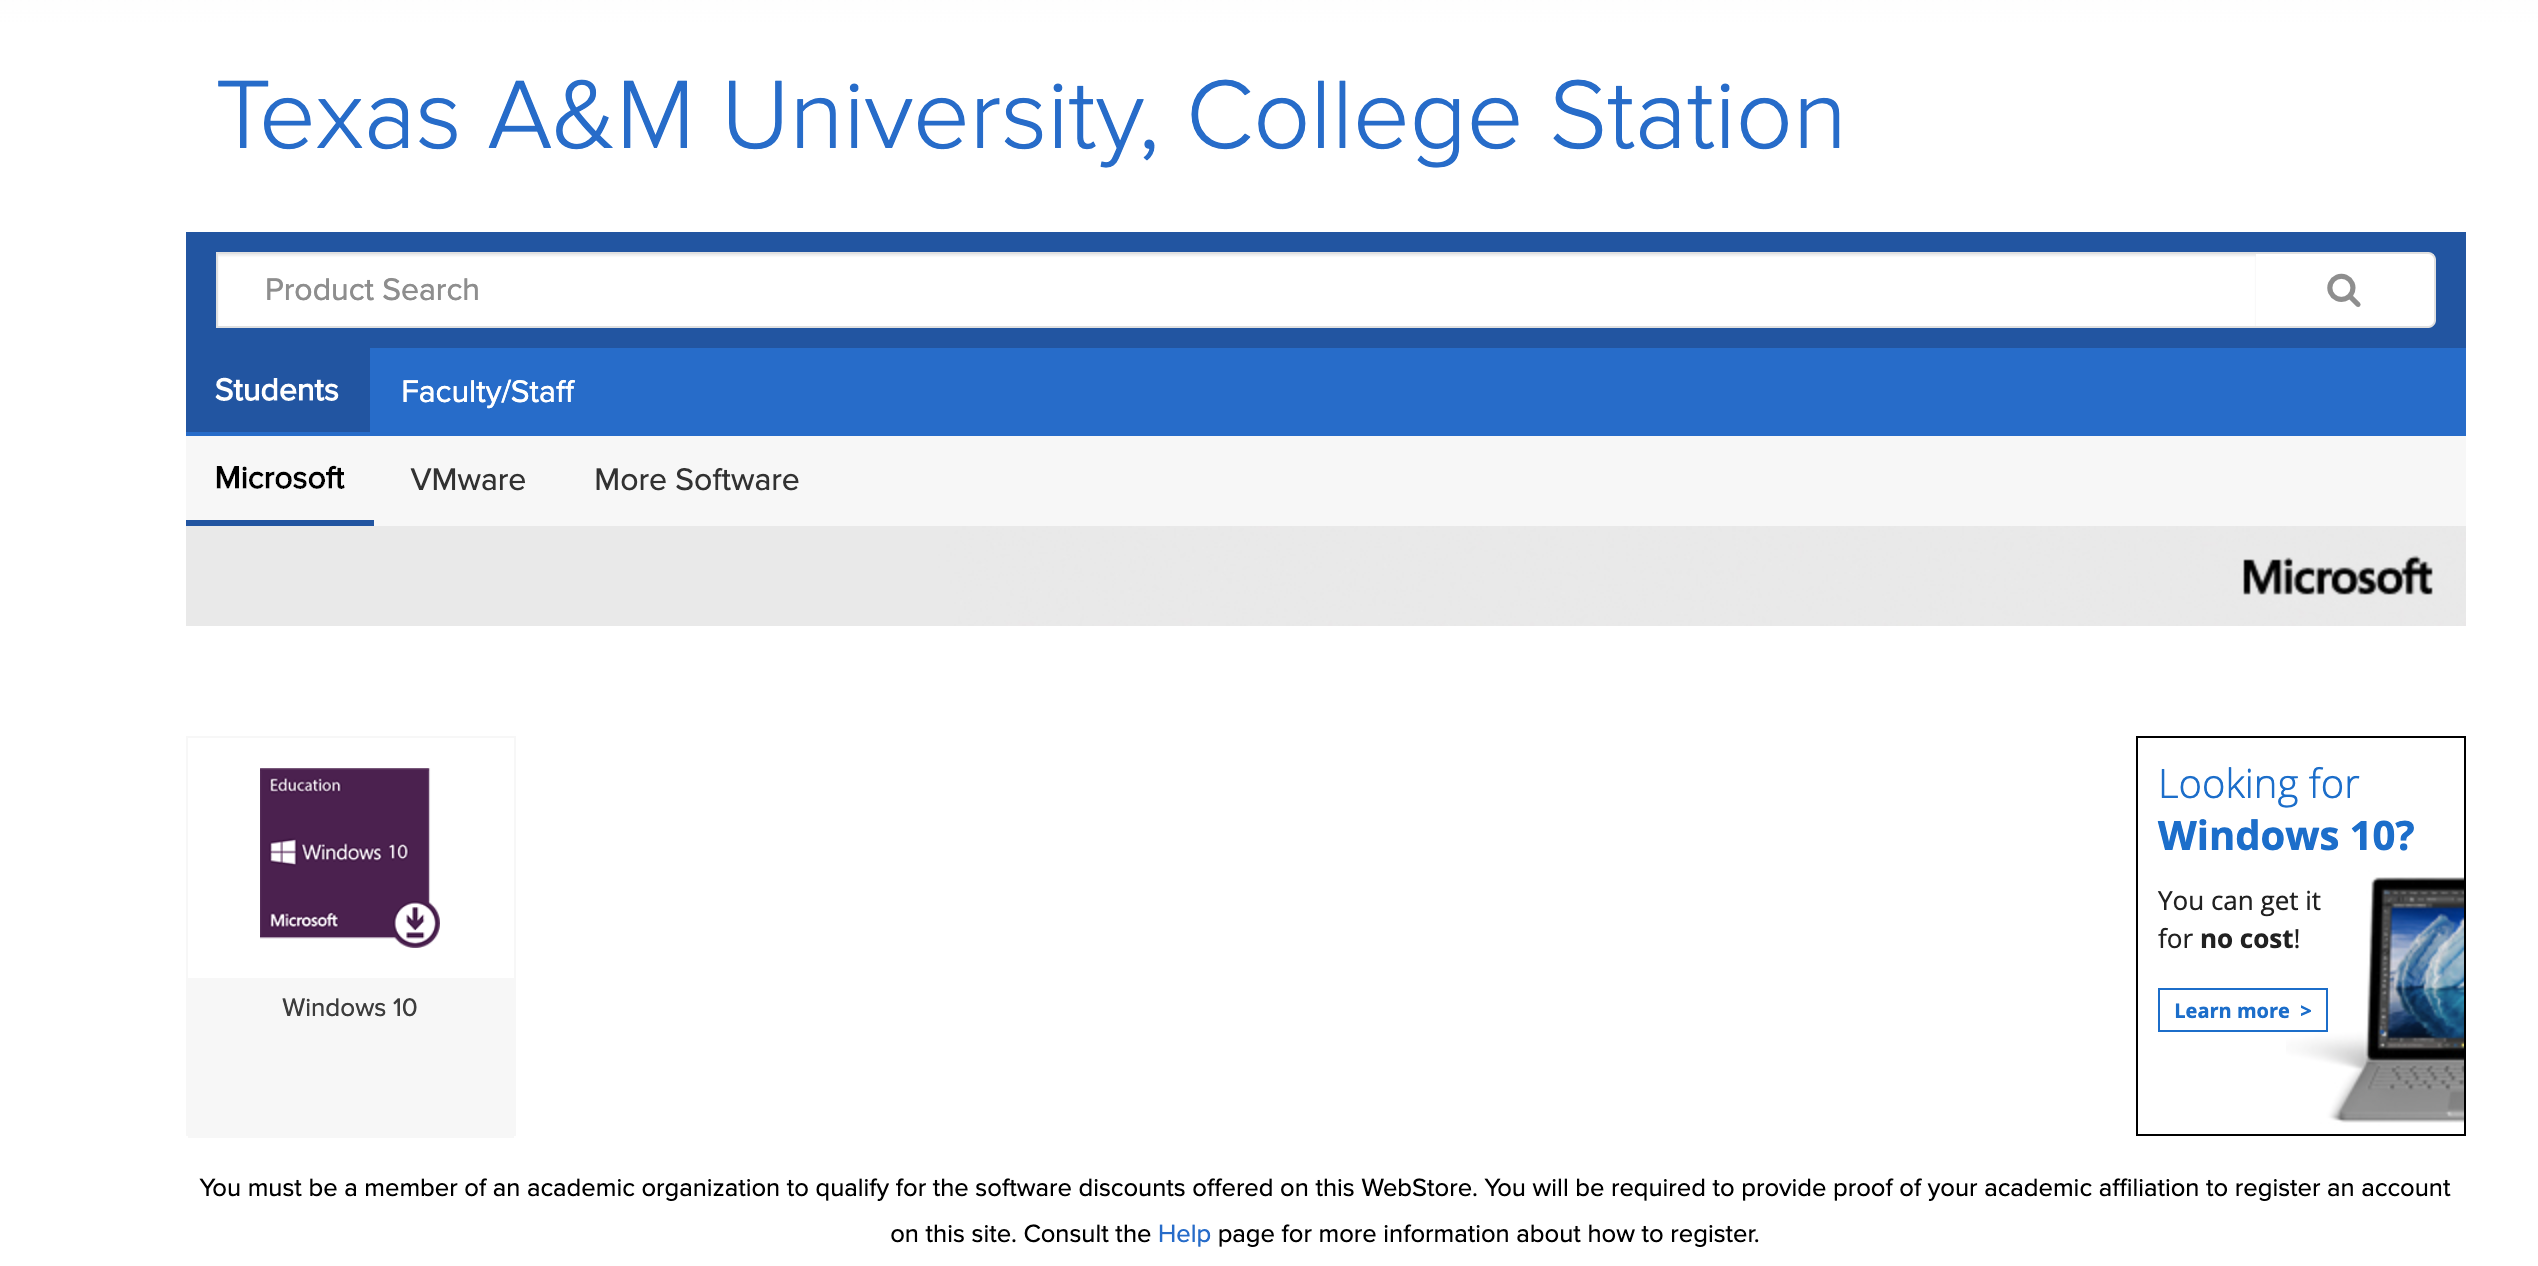
\includegraphics[ width=1\textwidth]{oth2}
	\caption{On The Hub Website}
	\label{oth2}
\end{figure}

To install Windows 10 you will need a copy of the Windows installation image (the ISO) and license key from Microsoft. As a student at Texas A\&M you can get a Windows 10 education license for free! Here are the steps involved to get your own copy of Windows 10:

\begin{enumerate}
    \item Navigate to https://software.tamu.edu/ in your favorite web browser
    \item On the right hand side of the screen you should see a link for requesting Microsoft software. A screenshot is shown in Figure~\ref{oth}. Click on the second "here"
    \item The link will take you to a website called "onthehub" where you can get your free copy of Windows 10. A screenshot is shown in Figure~\ref{oth2} 
    \item Select Windows 10 and complete the purchase (it's still a purchase, even though you are not paying anything) and you will be shown your Windows 10 license key. Make a careful note of this. After 30-days, this key will not be accessible from the website, so please store a copy for your records
    \item To download the ISO, go to the following website: 
    
    https://www.microsoft.com/en-us/software-download/vlacademicwindows10
    \item Select either the 32-bit or 64-bit version based on your Mac and download the ISO
    \item The file that you downloaded should end in a ".iso"
\end{enumerate}

\noindent
Now that you have your Windows 10 ISO and license key, let's get started with the installation process.



\section{Install Windows 10 using Boot Camp Assistant}
\begin{figure}[!h]
	\centering 
	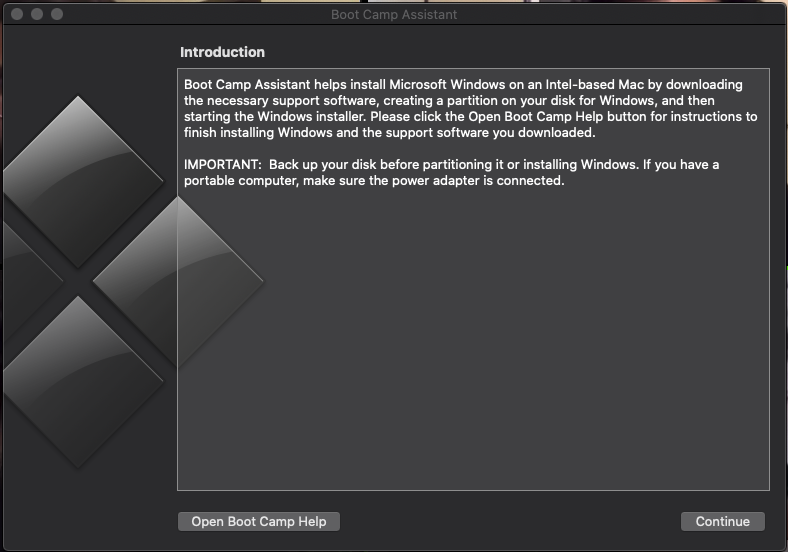
\includegraphics[ width=.5\textwidth]{bootcamp}
	\caption{Boot Camp Assistant}
	\label{bootcamp}
\end{figure}

\begin{figure}[!h]
	\centering 
	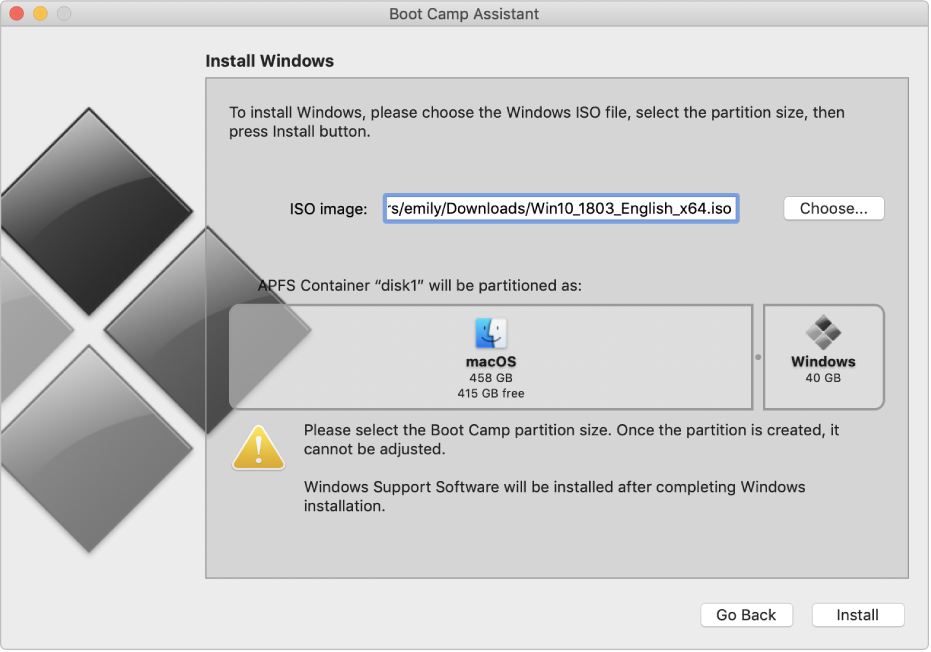
\includegraphics[ width=.8\textwidth]{new_size}
	\caption{Select ISO / Partition Size}
	\label{b2}
\end{figure}

\begin{figure}[!h]
	\centering 
	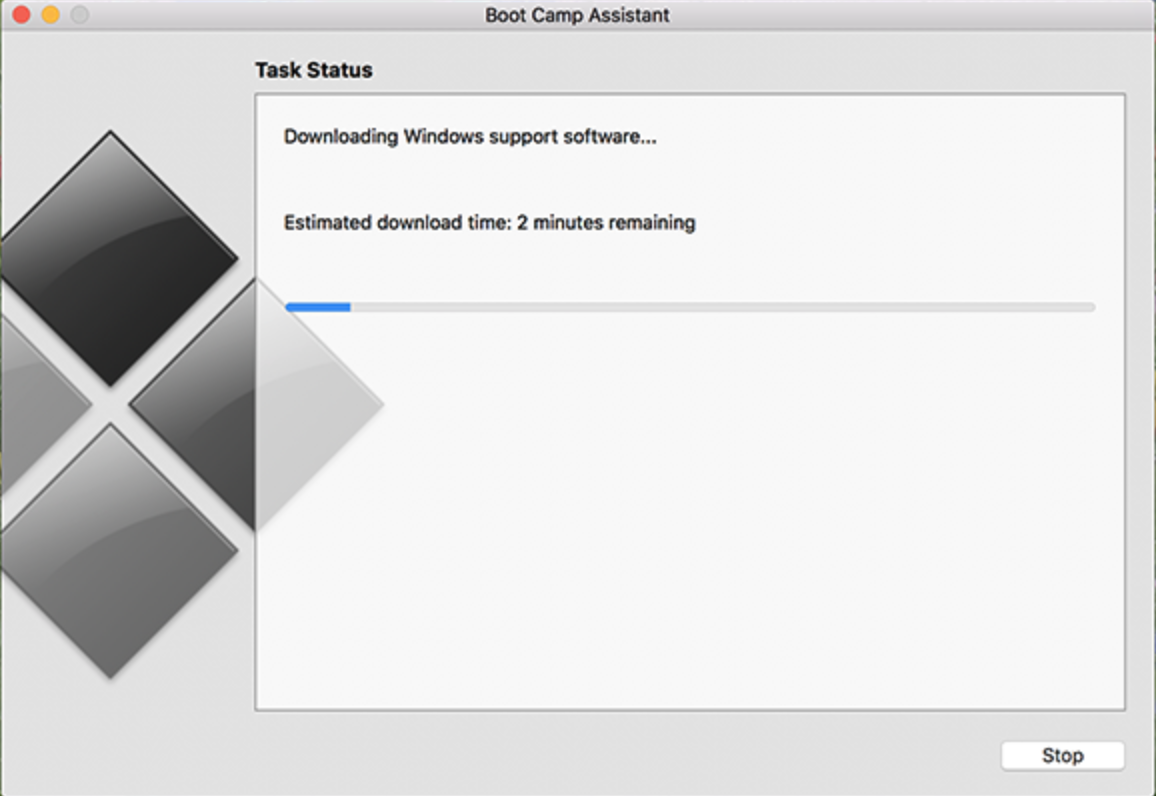
\includegraphics[ width=.8\textwidth]{sup2}
	\caption{Downloading Support Software}
	\label{sup}
\end{figure}

Before starting the installation, close all other programs on your Mac. Now to start Boot Camp, bring up the spotlight search by pressing Command+Space. Type "bootcamp" and double click on the first result. The first screen you see is shown in Figure~\ref{bootcamp}. Click on "continue".
\\
\\
\noindent
On the next screen, shown in Figure~\ref{b2}, you will need to select the ISO image that you just downloaded and set the partition size for Windows 10.  
\\
\\
\noindent
First, click on the "Choose" button and select the file that you just downloaded from the internet. Next, let's set our partition size. Use your mouse to click and drag the gray dot between "macOS" and "Windows" so that Windows has at least 128 GB (we recommend at least 128 GB). The space that you provision for Windows will not be available when you are using MacOS. Next Click Install. If you do not have 128 GB of free space available, select the largest size that you can (be careful, you want your MacOS to also have some free space).
\\
\\
Now you should see a screen that will say "Downloading Windows Support Software", shown in Figure~\ref{sup}. This step will take a while and at some point you will be prompted for your username and password, like in Figure~\ref{username}. Enter your credentials (the same ones you use to login on your Mac) and click OK.
\\
\\
\noindent
Boot Camp is now going to reboot your Mac and you will boot into the setup to install Windows 10. You will see the windows loading screen followed by "setup is starting" against a blue background. You will next be asked to select your Language, Time and Keyboard. The default options (and the ones we used) are shown in Figure~\ref{options}. Click "Next". 
\\
\begin{figure}[!h]
	\centering 
	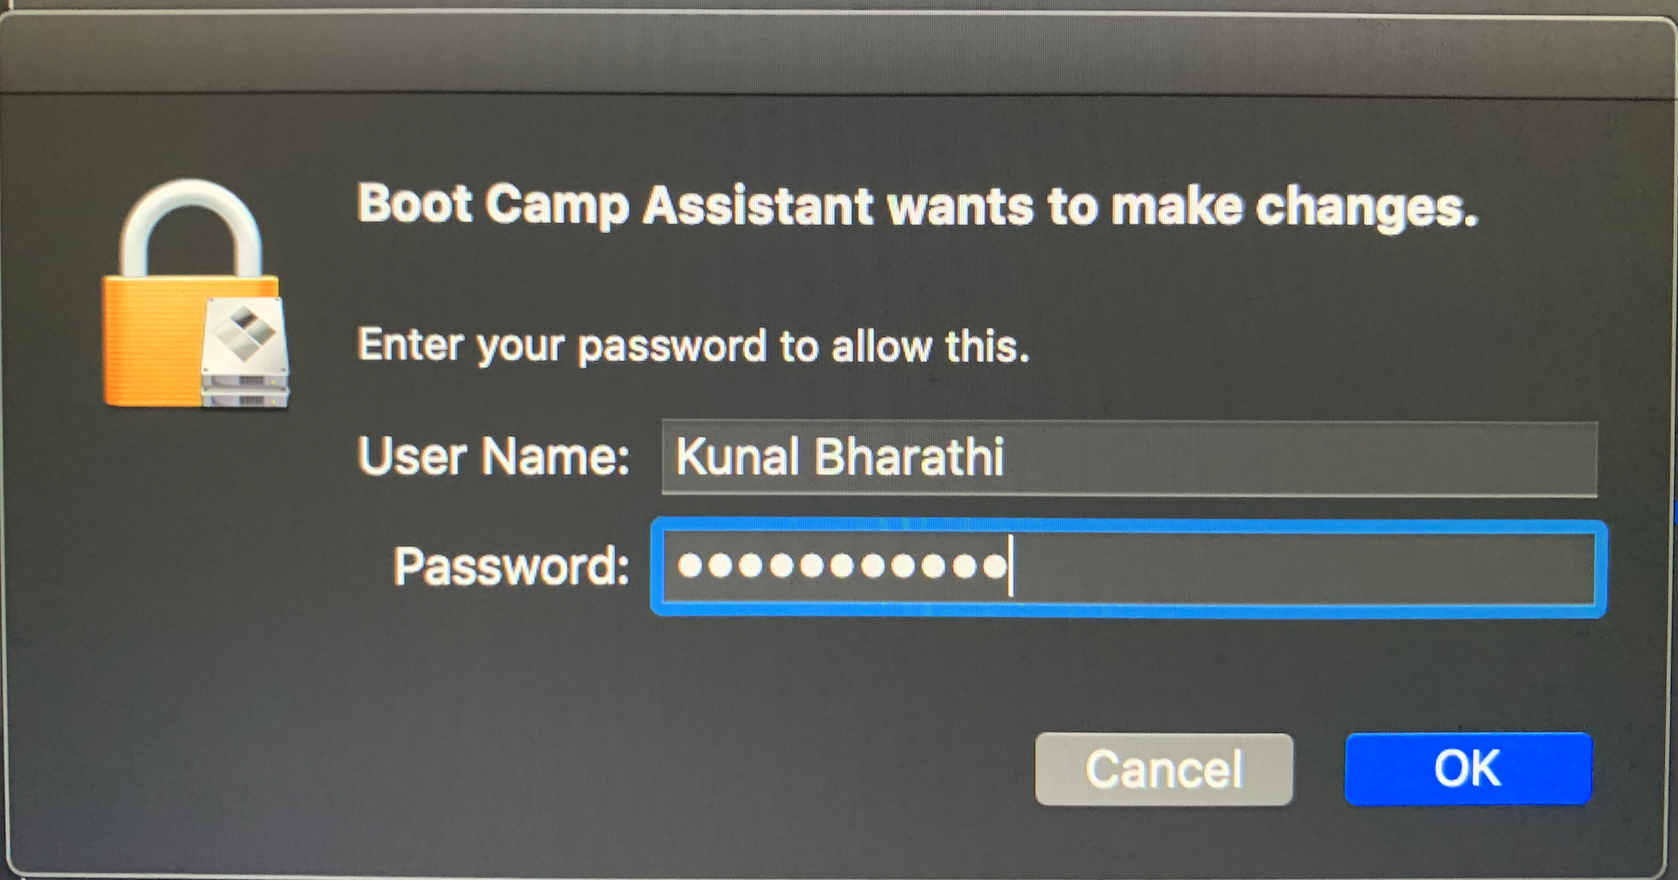
\includegraphics[ width=.5\textwidth]{username}
	\caption{Username/Password Prompt}
	\label{username}
\end{figure}

\noindent
The program will now ask you to enter your Windows 10 license key. Enter the license key you previously got in this tutorial in Section 2.3. Click "Next". Click "Next" on any other prompts and you should see the Windows installation process start. At the end of this process your computer will reboot again and Windows 10 will start.
\\
\\
\noindent
Since this is an educational copy of Windows 10, you will be asked to login. Use your TAMU email address to login. The login screen is shown in Figure~\ref{login}. The sign in procedure is similar to logging into Howdy with two-factor authentication. After you login successfully, Windows Hello will ask you to setup a PIN. This will make future logins faster. Click next to set your PIN. While setting up the pin, you will have to provide your phone number for verification. This screen is shown in Figure~\ref{phone}. Once you have added the phone verification, you can set your pin, and the screen looks like Figure~\ref{pin}.

% \begin{figure}[!h]
% 	\centering 
% 	
\includegraphics[ width=.8\textwidth]{start}
% 	\caption{Boot into Windows Setup}
% 	\label{start}
% \end{figure}


\begin{figure}[!h]
	\centering 
	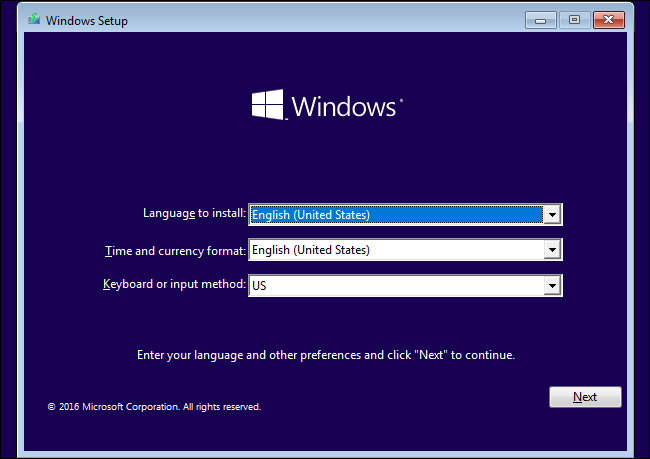
\includegraphics[ width=.5\textwidth]{win10start}
	\caption{Setup Options}
	\label{options}
\end{figure}

\begin{figure}[!h]
	\centering 
	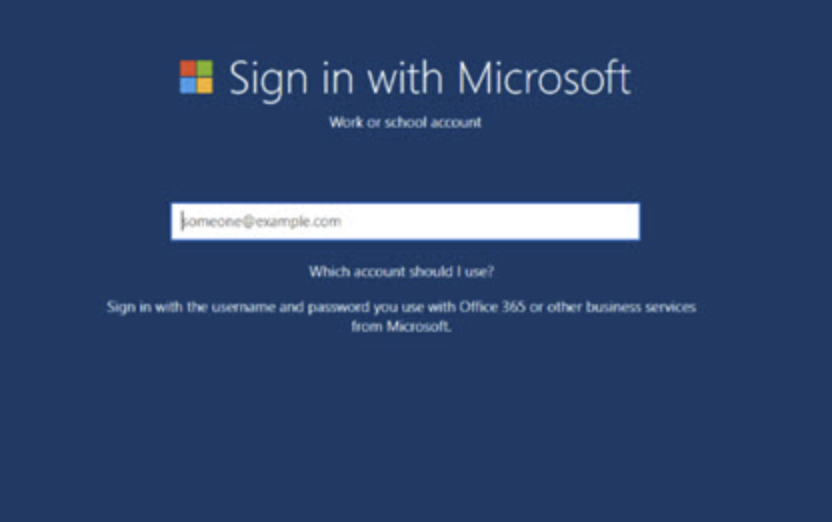
\includegraphics[ width=.5\textwidth]{login}
	\caption{Sign In With TAMU Account}
	\label{login}
\end{figure}

\begin{figure}[!h]
	\centering 
	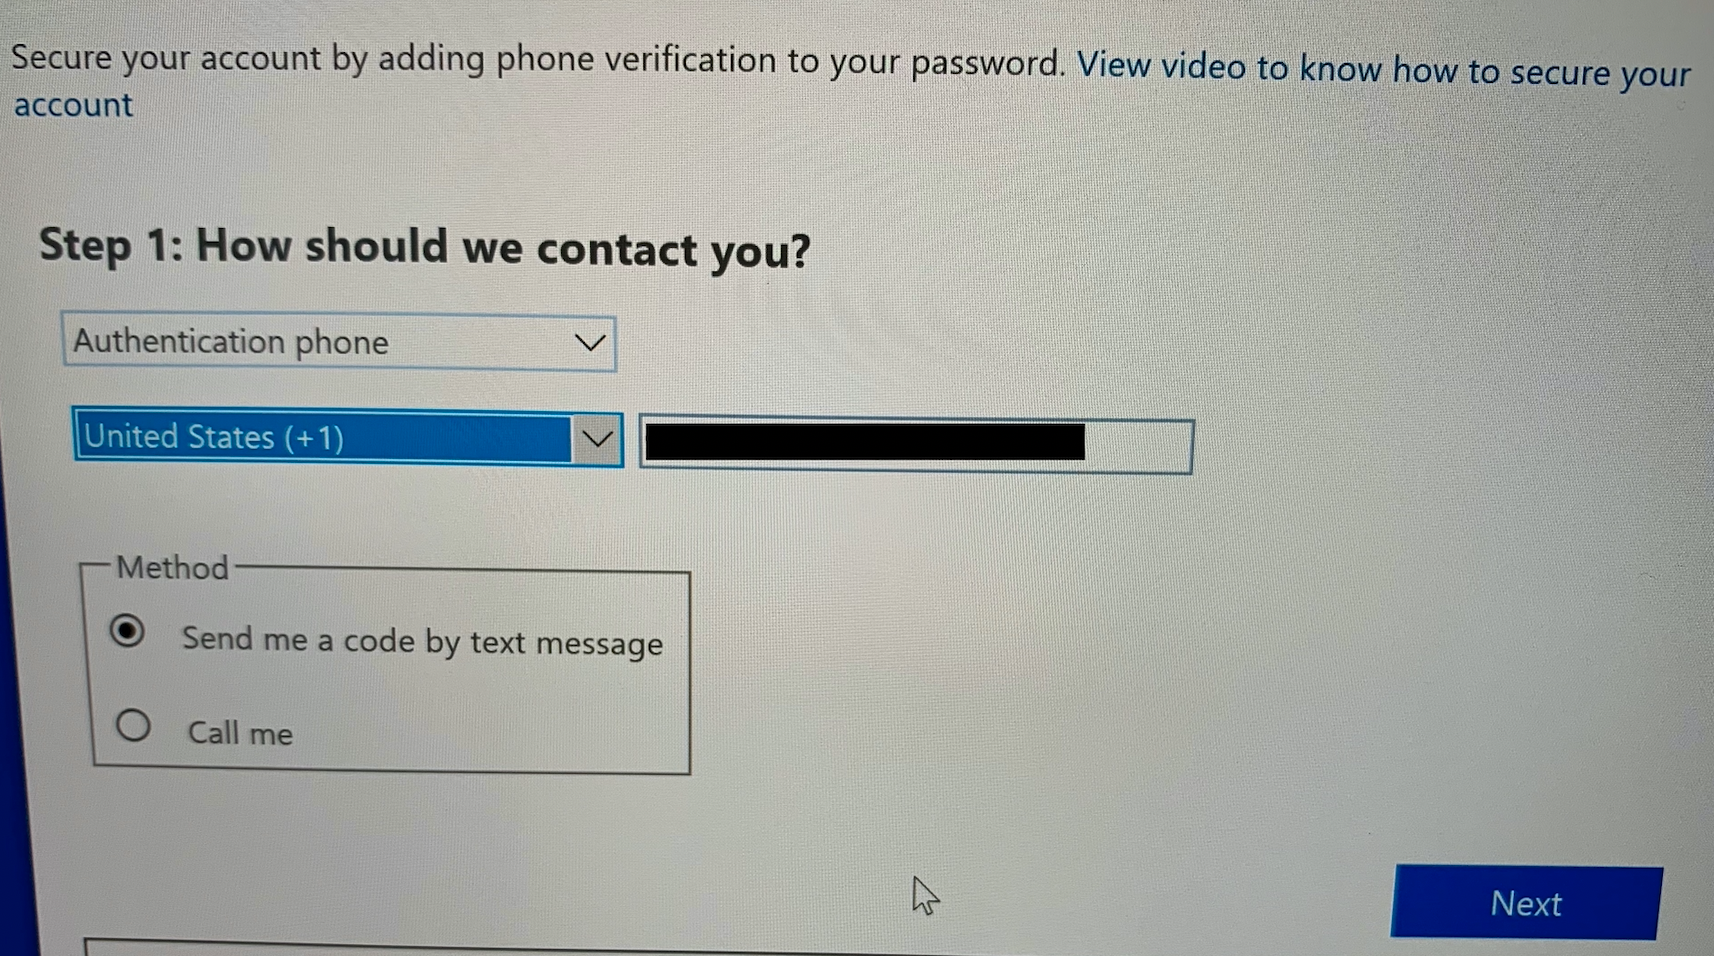
\includegraphics[ width=.5\textwidth]{phone}
	\caption{Setting Up Your Windows Hello Pin - 1}
	\label{phone}
\end{figure}

\begin{figure}[!h]
	\centering 
	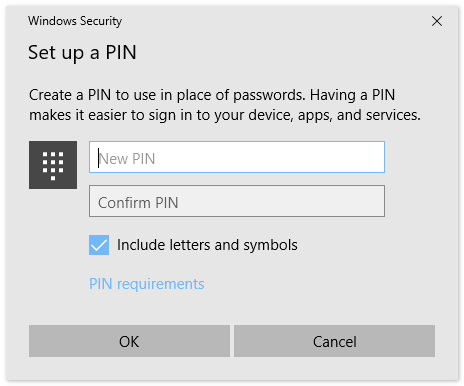
\includegraphics[ width=.3\textwidth]{pinsetup}
	\caption{Setting Up Your Windows Hello Pin - 2}
	\label{pin}
\end{figure}

\noindent
There is one last step before your Windows installation is complete. At this point in the process, you should be able to login in to Windows 10. The first time you login, do not do anything until the Boot Camp drivers are installed. On your first login, after the Windows 10 desktop loads,  you will see the the Boot Camp driver installation program shown in Figure~\ref{driver}. Click Next and complete the installation. Keep "Restart Now" selected as shown in Figure~\ref{restart} and click on finish. Your Mac will now reboot and take you to the windows login screen. Use your Windows Pin to login to your account.

That's it! You have successfully installed Windows 10 on your Mac.

\begin{figure}[!h]
	\centering 
	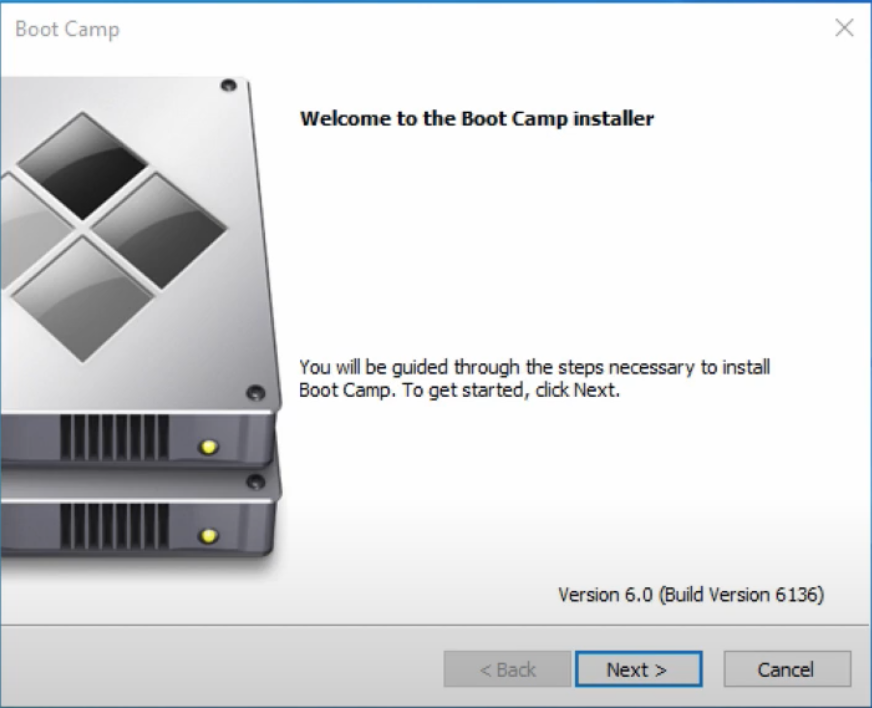
\includegraphics[ width=.3\textwidth]{winb1}
	\caption{Boot Camp Installer}
	\label{driver}
\end{figure}

\begin{figure}[!h]
	\centering 
	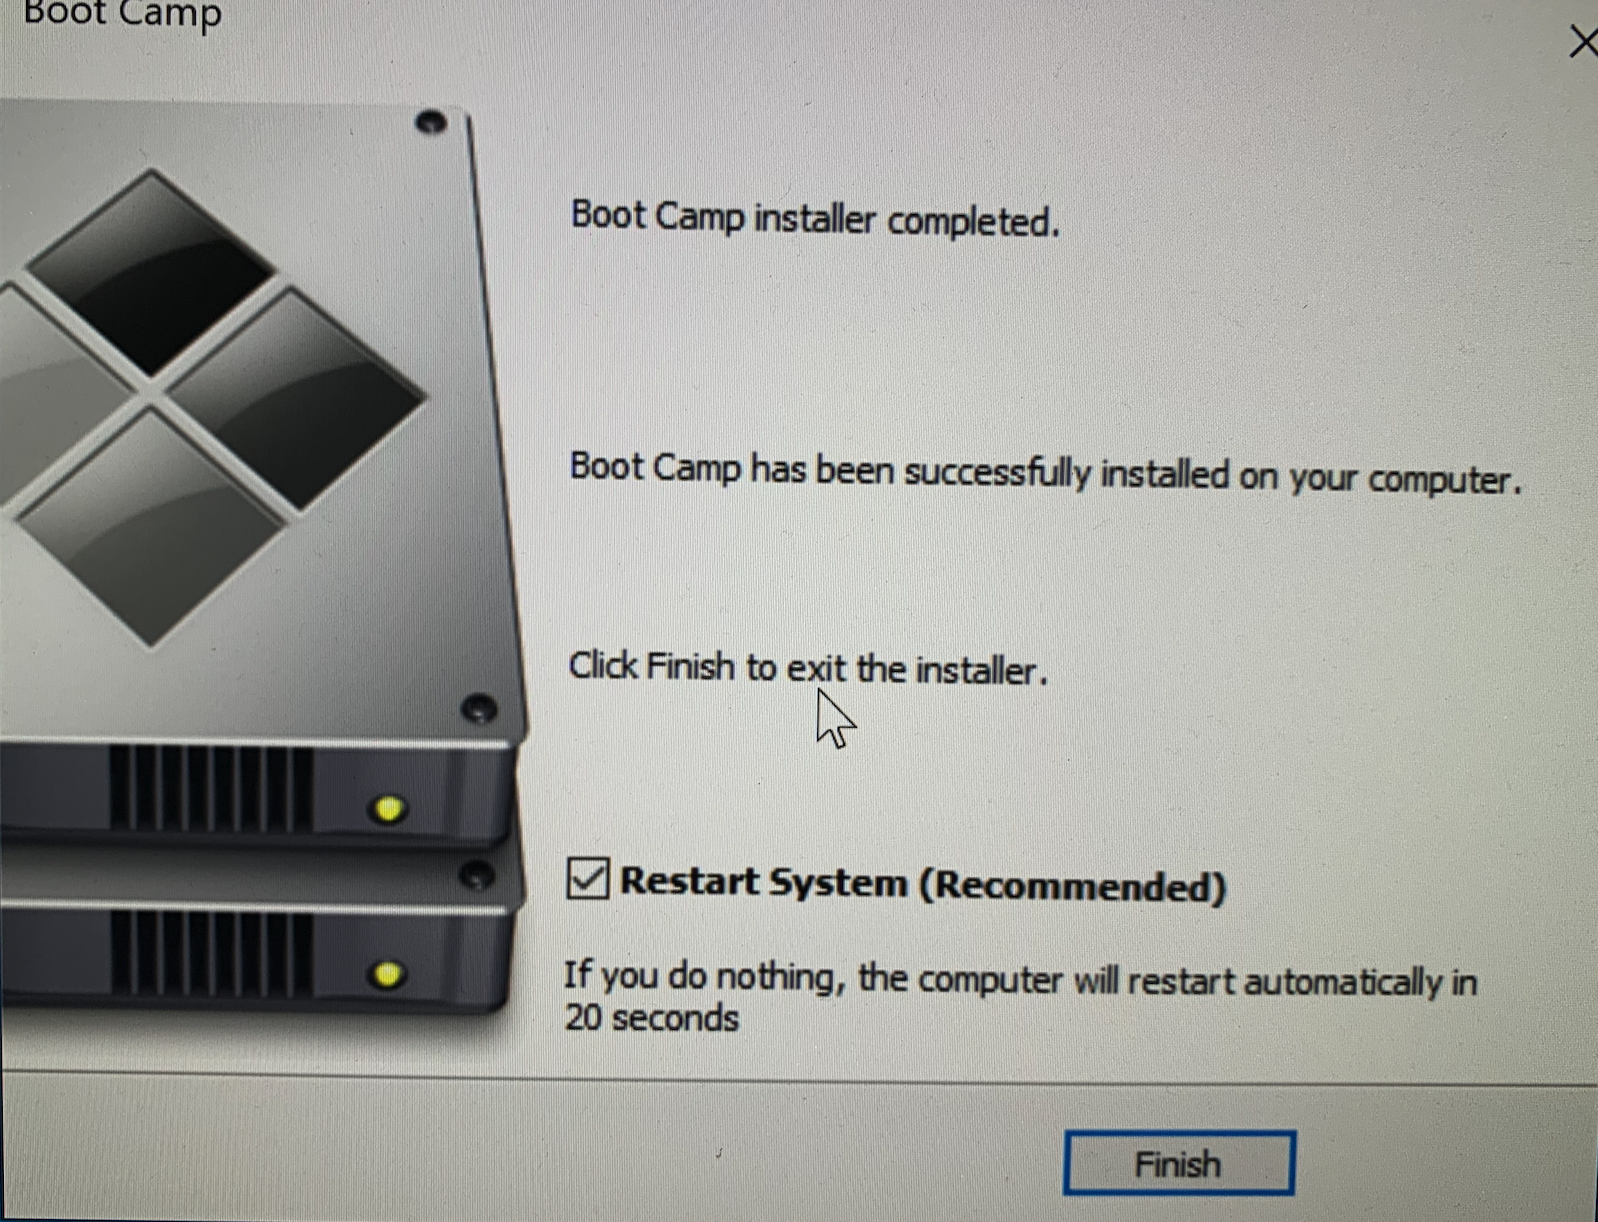
\includegraphics[ width=.3\textwidth]{restart}
	\caption{Boot Camp Installer - Finish}
	\label{restart}
\end{figure}

\section{Working with Mac and Windows}

Now that you have installed Windows on the same system as MacOS, it is easy to switch between the 2 operating systems. To switch from MacOS to Windows, restart your computer while holding down the OPTION key. Your computer will give you an option to either boot into MacOS or into Windows. The same works when powering on the computer. Holding the OPTION key while powering on the system will give you an option to select which operating system to boot into.

\end{document}
